%  %*----------- SLIDE -------------------------------------------------------------
%  \begin{frame}[t]{Linha de pesquisa} 

%     No RASC existem diversos projetos de diferentes vertentes da área da robótica, sendo uma delas a dos manipuladores.

%     \vspace*{0.3cm}

%     A linha de pesquisa dos manipuladores busca desenvolver pesquisas relacionadas a controle, cinemática e aplicações destes sistemas robóticos.

%     \vspace*{0.3cm}

%     Os grupos de pesquisa que compõem essa trilha dos manipuladores são:

%     % \vspace*{0.8cm}
%     % 
\includegraphics[width=1\textwidth]{equipe.png}
% %*----------- notes
%     \note[item]{Notes can help you to remember important information. Turn on the notes option.}
% \end{frame}
% %-
%*----------- SLIDE (IMAGEM DO PROJETO) -------------------------------------------------------------
\begin{frame}[t]{Projetos da linha de pesquisa }
    \begin{figure}
        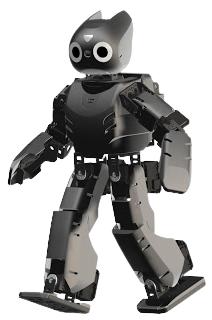
\includegraphics[width=0.8\textwidth]{darwin.png}
        %\caption{.}
    \end{figure}
\end{frame}
  %*----------- SLIDE (ANDAMENTO DO PROJETO) -------------------------------------------------------------
  \begin{frame}[c]{Andamento do projeto}
    \begin{table}[ht!]
        %\centering
            \caption{Lista de robôs}
            \begin{tabular}{|c|c|c|c|} \hline
                \textbf{Atividade}&\textbf{Status}&\textbf{Atividade}&\textbf{Status}\\\hline
                Walker           &Em andamento &  Arbotix & S/ uso\\ \hline
                Horta-bot        &Em andamento &  Ergo & S/ uso\\ \hline
                DOBOT Magician   &Em andamento &  Borg  & Utilizado\\ \hline
                OPEN Manipulator &Utilizado       &  JeRotimon & Utilizado\\ \hline
            \end{tabular}
        \end{table}
        \begin{table}[ht!]
            %\centering
                \caption{ATIVIDADES do WARTHOG+AUM}
                \begin{tabular}{|c|c|c|c|} \hline
                    \textbf{Atividade}&\textbf{Status}&\textbf{Atividade}&\textbf{Status}\\\hline
                    Bomb Mission Fase 1 &Finalizado & Algoritmo preditor  &Finalizado\\ \hline
                    Bomb Mission Fase 2 &Em andamento & DOE solucionadores &Pausado\\ \hline
                \end{tabular}
            \end{table}
%*----------- notes
    \note[item]{Notes can help you to remember important information. Turn on the notes option.}
\end{frame}
%-


%*----------- SLIDE -------------------------------------------------------------
\begin{frame}[c]{} 
    % \transdissolve[duration=0.5]
   
    \begin{center}
        \Wider{%
        \begin{shaded}
        \begin{center}
            \vspace*{0.3cm}
            \resizebox{!}{0.6cm}{%
                Projetos centrais
            }%
        \end{center}
        \end{shaded}
        }%
    \end{center}
       
%*----------- notes
    \note[item]{Notes can help you to remember important information. Turn on the notes option.}
\end{frame}
%
%*----------- SLIDE -------------------------------------------------------------
\begin{frame}[t]{Warthog + AUM} 

    O projeto \textbf{Warthog + AUM} consiste na integração de um robô manipulador com o robô UGV Warthog.

    \vspace*{0.3cm}
    %\newline
        \begin{columns}[t]
            \column{.05\linewidth}
            \column{.4\linewidth}
            \begin{center}
                Este sistema permitiu o desenvolvimento de alguns \textbf{desafios} e \textbf{implementações} utilizando diferentes modelos de manipuladores.
            \end{center}
            \column{.6\linewidth}
            \begin{center}
            %\centerline{
                \begin{figure}
                    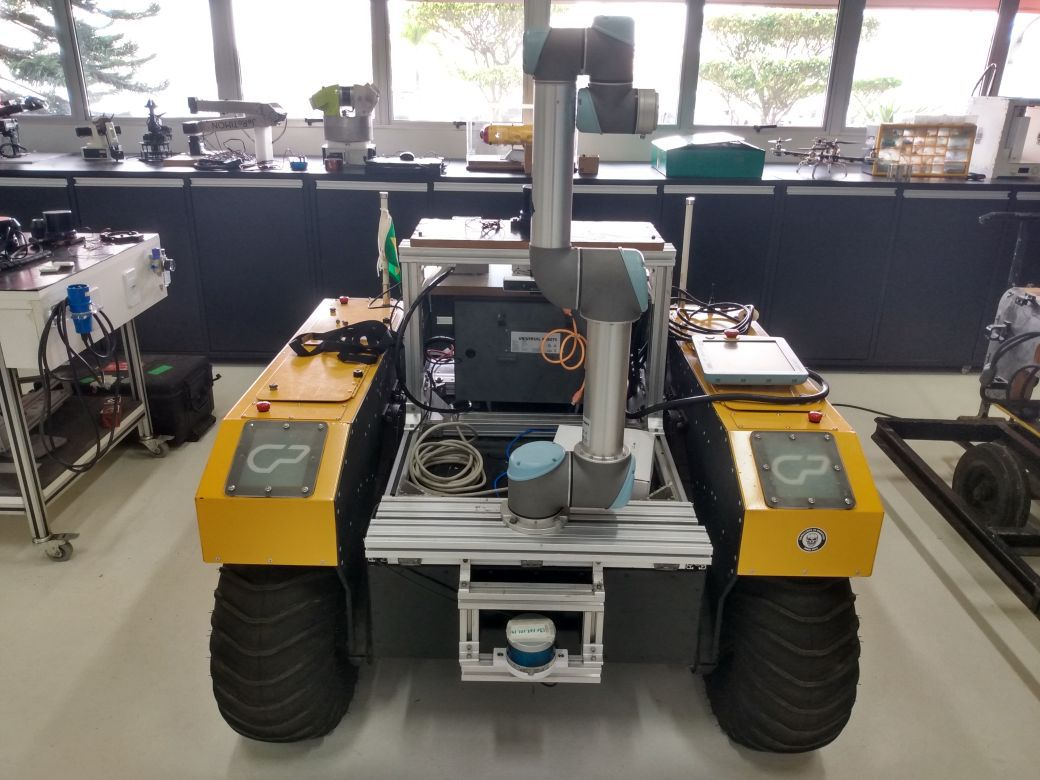
\includegraphics[width=.65\textwidth]{warthog+aum/full-system.jpg}
                    %\caption{Pista de corrida \cite{agostini2007}}
                \end{figure}
            %}
            \end{center}
        \end{columns}
%*----------- notes
    \note[item]{Notes can help you to remember important information. Turn on the notes option.}
\end{frame}
%-

%*----------- SLIDE -------------------------------------------------------------
\begin{frame}[t]{Bomb Mission - Fase 1} 
    \framesubtitle{Warthog + AUM}

    \textbf{Objetivo:} Realizar o desarme de uma bomba fictícia. Para isso, o robô deve navegar de forma autônoma e reconhecer as cores da bomba através de visão computacional.

    \vspace*{0.3cm}
    %\newline
        \begin{columns}[t]
            \column{.05\linewidth}
            \column{.4\linewidth}
            \vspace*{0.8cm}

            \textbf{O que foi feito:} 
            % \begin{center}
             Este desafio foi realizado pela primeira 
             turma dos bolsistas utilizando o Jerotimon.
            % \end{center}
            \vspace*{0.5cm}

            \textbf{Status:} Finalizado
            \column{.6\linewidth}
            \begin{center}
            %\centerline{
                \begin{figure}
                    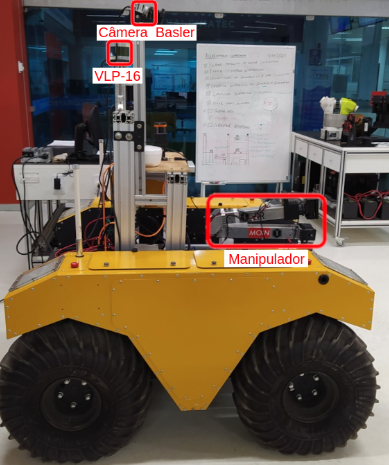
\includegraphics[width=.41\textwidth]{jerotimon.png}
                    %\caption{Pista de corrida \cite{agostini2007}}
                \end{figure}
            %}
            \end{center}
        \end{columns}
%*----------- notes
    \note[item]{Notes can help you to remember important information. Turn on the notes option.}
\end{frame}
%-
%*----------- SLIDE -------------------------------------------------------------
\begin{frame}[t]{Bomb Mission - Fase 2} 
    \framesubtitle{Warthog + AUM}

    \textbf{Estado atual:} Estava programado para ser iniciado pela turma atual, utilizando o Borg considerando fazer um comparativo entre a state-machine e o behavior-tree.

    \vspace*{0.3cm}
    %\newline
        \begin{columns}[t]
            \column{.05\linewidth}
            \column{.4\linewidth}

            \textbf{O que foi feito:}
            \begin{itemize}
                \item Instalação do Borg na estrutura do Warthog.
                \item Atualizado o modelo do robô na simulação.
            \end{itemize}
            % \end{center}
            \vspace*{0.5cm}

            \textbf{Status:} Em andamento
            \column{.6\linewidth}
            \begin{center}
            %\centerline{
                \begin{figure}
                    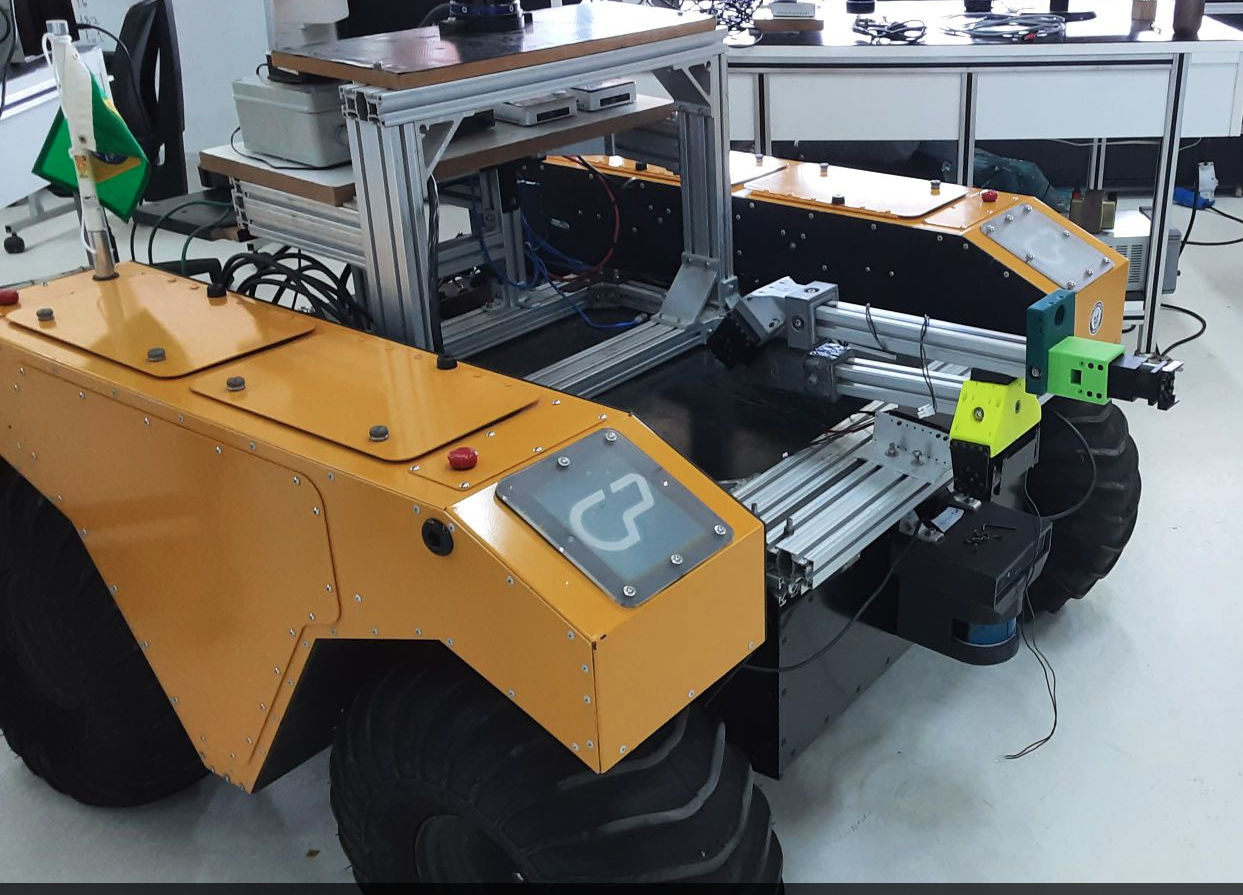
\includegraphics[width=.6\textwidth]{borg.png}
                    %\caption{Pista de corrida \cite{agostini2007}}
                \end{figure}
            %}
            \end{center}
        \end{columns}
%*----------- notes
    \note[item]{Notes can help you to remember important information. Turn on the notes option.}
\end{frame}
%-
%*----------- SLIDE -------------------------------------------------------------
\begin{frame}[t]{Aplicações com o UR5} 
    \framesubtitle{Warthog + AUM}
    %\newline
        \begin{columns}[t]
            \column{.05\linewidth}
            \column{.4\linewidth}
            \vspace*{-0.3cm}

            \textbf{DOE Planejadores:}
            \begin{itemize}
                \item Foram obtidos os dados dos testes.
                \item Faltou realizar a análise e desenvolver um artigo.
                \item \textbf{Status:} Em pausa
            \end{itemize}
            \vspace*{0.3cm}

            \textbf{Algoritmo Preditor:}
            \begin{itemize}
                \item Algoritmo utilizando filtro de Kalman.
                \item \textbf{Status:} Finalizado
            \end{itemize}
            % \end{center}
            \column{.6\linewidth}
            \begin{center}
            %\centerline{
                \begin{figure}
                    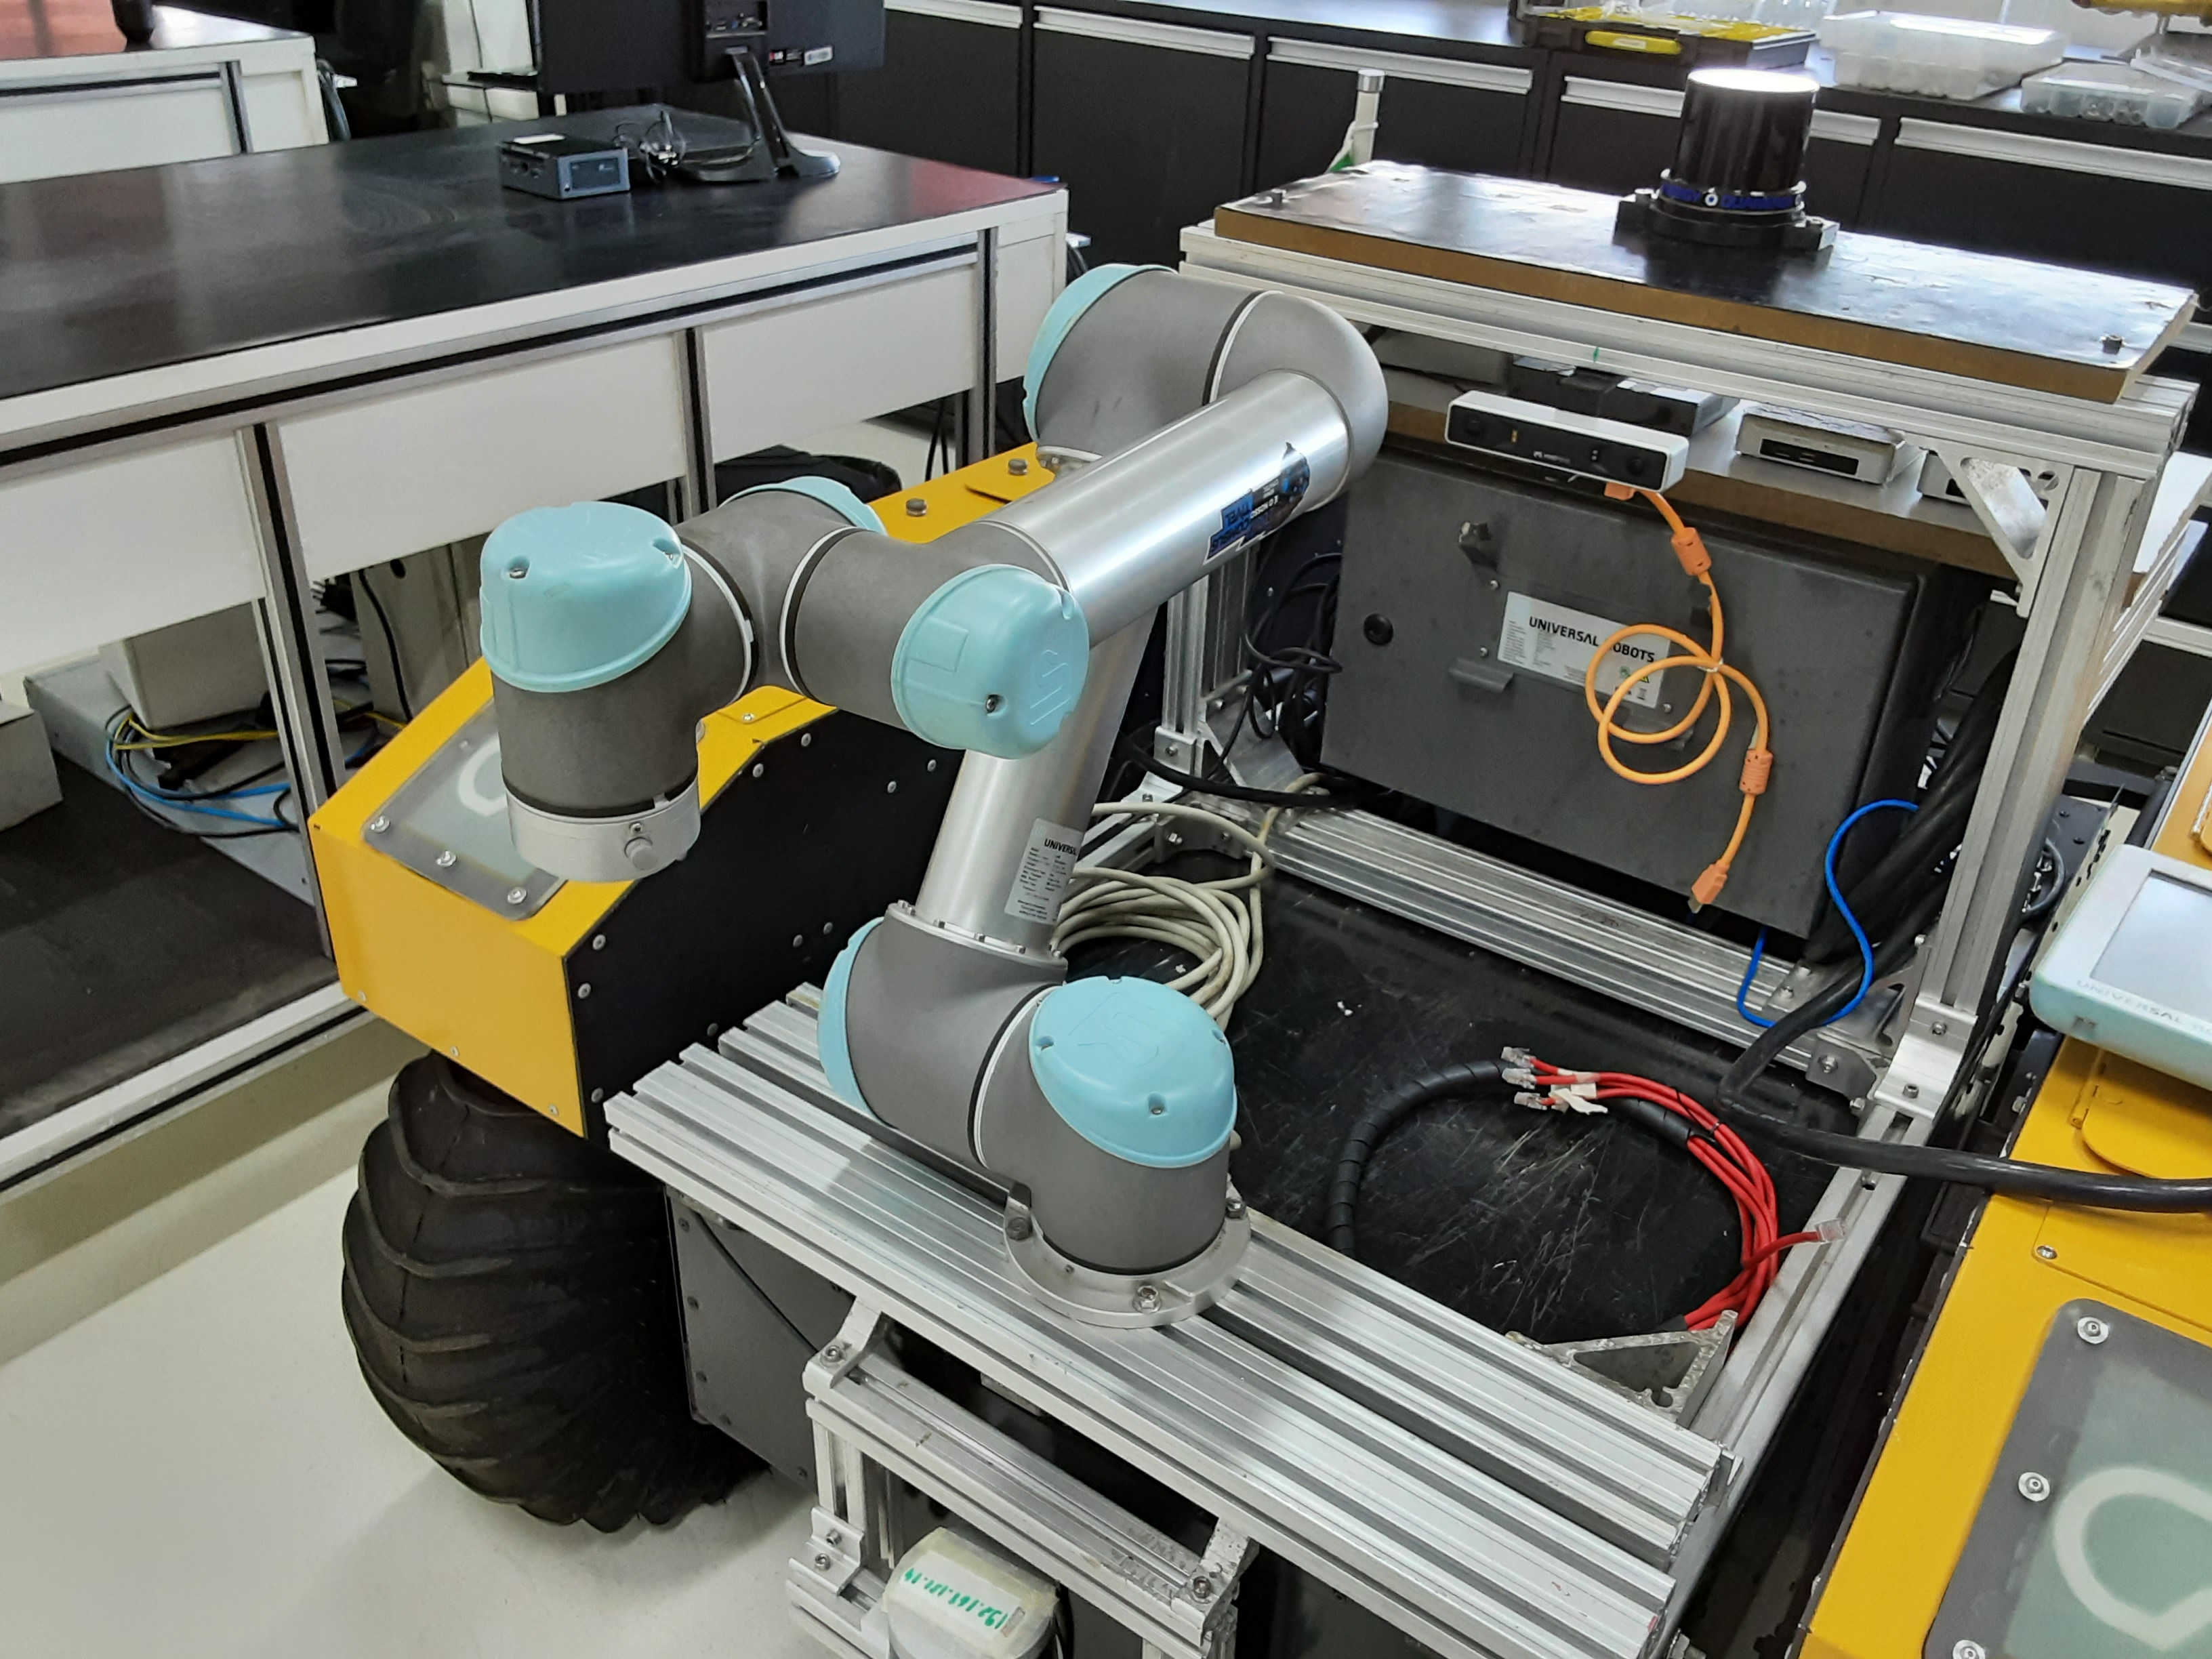
\includegraphics[width=.6\textwidth]{ur5.jpg}
                \end{figure}
            %}
            \end{center}
        \end{columns}
%*----------- notes
    \note[item]{Notes can help you to remember important information. Turn on the notes option.}
\end{frame}
%-